\Chapter{Felhasznált technológiák és fejlesztői környezetek}

A következőkben bemutatásra kerülnek azok a technológiák és fejlesztői környezetek, amiket használni fogok a fejlesztéshez.

\Section{Backend}

A backend a webalkalmazás szerver oldala, amit nem lát a felhasználó. Itt szokott történni az adatbázissal való kommunikáció, továbbá az authentikáció (hitelesítés) és az authorizáció (engedélyezés). Nagyon sokféle backend technológia létezik, mint például: PHP, Python, JavaScript és Java programozási nyelvek. A Java-t fogom használni a fejlesztések során.

\subsection{Java}

A Java \cite{Java} egy objektum orientált programozási nyelv, amit James Gosling fejlesztett a ’90-es években Sun Microsystemsnél. Eredetileg interaktív televíziózásra készült, de akkoriban túl fejlett volt digitális kábeltelevíziós ipar számára.

A Java célja a hordozhatóság, ami azt jelenti, hogy a Java-ban írt programoknak hasonlóan kell futnia bármely JRE-vel rendelkező operációs rendszeren. Java nyelvi kódot először bájtkódra fordítják, ami hasonló a gépi kódhoz, de virtuális gép általi végrehajtásra készülnek. Vannak mikro vezérlők amik képesek a Java bájtkódját közvet-
lenül hardveren futtatni.

A Java a szintaxisát a C és C++ nyelvből örökölte. A Java nem támogatja az operátor túlterhelést vagy a többszörös öröklődést (interfészek esetében lehetséges).

A Java jelenlegi tulajdonosa az Oracle Corporation 2010-óta, miután felvásárolta a Sun Microsystems-t.

A Java az egyik legelterjedtebb programozási nyelv, mivel az elterjedt operációs rendszerekre tudunk vele alkalmazást fejleszteni, és a tervezésnél az volt a cél, hogy könnyen tanulható legyen.

\subsection{Spring Boot}

A Spring egy Java alapú webalkalmazás-keretrendszer, ami nyílt forráskódú, és a Spring Boot egy Spring-keretrendszerre épülő bővítmény. A Spring testreszabott webalkalma-
zások létrehozásához tökéletes, ami teljesen konfigurálható az előre elkészített fügvény-
könyvtárakkal. Spring Boot-tal különálló Spring alkalmazásokat hozhatunk létre, amit azonnal futtathatunk.

A Spring Boot használata nagyon egyszerű, jó minőségű alkalmazásokat lehet benne fejleszteni kevesebb fejlesztési idő alatt. Beépített HTTP-kiszolgálókat tartalmaz, mint a Tomcat és a Jerry.

A Spring Boot tartalmaz egy Maven-hez tartozó \textit{(pom.xml)} fájlt, amiben \textit{spring-boot-dependency}-ket tudunk megadni, mint például:

\begin{itemize}
\item \textit{spring-boot-starter-web},
\item \textit{spring-boot-starter-data-jpa},
\item \textit{spring-boot-starter-test}.
\end{itemize}

A \textit{pom.xml} egy konfigurációs fájlként is használható.

Spring initializr: A Segítségével könnyedén „összerakhatjuk” a projektünk alapját, megadhatunk például függőségeket, megadhatjuk, hogy milyen programozási nyelven szeretnénk elkészíteni, a projekt nevét \cite{SpringBoot}.

\Section{Adatbázis}
Az adatbázis nem más, mint elektronikusan tárolt adatok, amik rendszerezve vannak. Segíti, hogy az adatok könnyebben és gyorsabban elérhetőek legyenek. Több fajta adatbázis is elérhető.


\subsection{PostgreSQL}

A PostgreSQL \cite{PostgreSQL} egy nyílt forráskódú relációs adatbáziskezelő rendszer, ami az egyik legrégebbi relációs adatbázis, nem mellesleg ingyenes. A relációs adatbázisok relációs modellen alapulnak. A relációs modell az adatokat egy vagy több sorból és oszlopból álló táblázatba (relációba) rendezi, és minden sorhoz rendel egy egyedi kulcsot.

A PostgreSQL a Kaliforniai egyetem Ingres projektjéből fejlődött ki. Az elterjedtebb operációs rendszerekkel kompatibilis. Támogatja a relációs és a nem relációs lekérdezé-
seket is, így JSON vagy SQL alapú útvonal-kifejezésekkel is elérhetőek az adatok.  Mind ezek miatt az egyik legnépszerűbb adatbázismotor (\ref{fig:Adatbázisok}. ábra).

\begin{figure}[h]
\centering
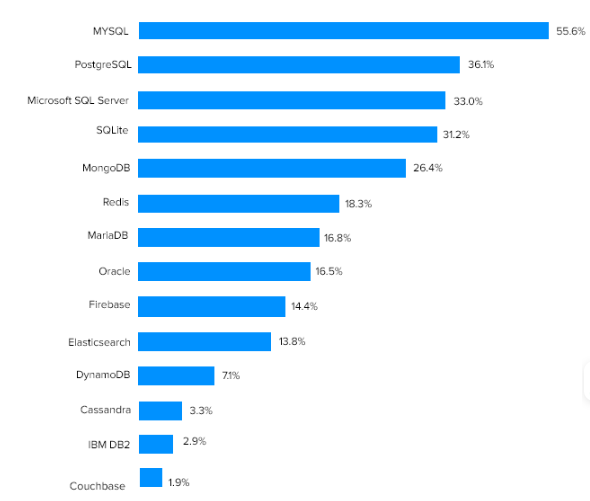
\includegraphics[scale=0.6]{images/top14_database.png}
\caption{A 14 legnépszerűbb adatbázis az Appinventiv kimutatása alapján \cite{databases}}
\label{fig:Adatbázisok}
\end{figure}
\newpage

\Section{Frontend}

A frontend a szoftver megjelenítési rétege. A weboldalnak azon rétege, amit a felhaszná-
ló is lát, és interakcióba tud vele lépni. Legfontosabb része a HTML (HyperText Markup Language), ez adja meg a weboldal kinézetének a vázát, és hozzá csatlakozik a CSS (Cascading Style Sheets), ami segítségével egyedi megjelenést biztosíthatunk a weboldalunknak. Több fajta keretrendszer létezik Frontend fejlesztésre, mint például:

\begin{itemize}
\item React,
\item Angular,
\item Vue.js.
\end{itemize}


\subsection{Angular}

Az Angular \cite{Angular} egy TypeScript-alapú, nyílt forráskódú webalkamazás-keretrendszer. 2016-ban jelent meg az első verzió.

A HTML sablon lehetővé teszi dinamikus értékek beszúrását, mint például szöveges értékek. Az Angular tartalmaz komponenseket, amelyek NgModulokba vannak rendez-
ve. Ezek a komponensek egyben tartalmazzák a TypeScript osztályt HTML-sablont stílusokkal. Minden alkalmazásnak van egy úgynevezett gyökérmodulja, aminek a neve általában az AppModule, amely a bootstrap mechanizmust biztosítja, amely elindítja az alkalmazást. Ngmodulok is importálhatnak más Ngmodulokat, például az útválasztó szolgáltatás használatához a Router NgModul-t.  Minden Angular alkalmazásnak van egy gyökérkomponense, ami összekapcsolja a komponens hierarchiát. Mindegyik kom-
ponenshez tartozik egy HTML-sablon, amely segítségével megjeleníthető a tartalom. Tartalmaz egy \textit{services} osztályt is. Ezt akkor használjuk, ha van olyan adat vagy logika, amelyek nem kapcsolódnak, de meg szeretnénk osztani a komponensek között.

\Section{Fejlesztői környezetek és fejlesztéshez használt p-
rogramok}

Egy alkalmazás fejlesztését nagyban megkönnyítik a fejlesztői környezetek és a fej-
lesztéshez használható programok.
\subsection{Intelij IDEA}

Az InteliJ IDEA \cite{Intelij} egy integrált fejlesztői környezet \cite{Intelij2}, amit a JetBrains fejlesztett ki. Ebben az IDEA-ban Java, Kotlin, Groovy és más JVM alapú nyelveken írt szoftvere-
ket lehet fejleszteni. (Az integrált fejlesztői környezet (IDE)  egy olyan  szoftveralkama-
zás, amely átfogó lehetőségeket biztosít a számítógép programozóknak a szofverfejlesz-
téshez.) Az IDE általában legalább egy forráskódszerkesztőből, építési autómatizálási eszközökből, és egy hibakeresőből áll. Egyes IDE-k, például a NetBeans és az Eclipse tartalmazzák a szükséges fordított, értelmezőt vagy mindkettőt; mások, például a SharpDevelop és a Lazuras nem.

Az InteliJ IDEA látható a \ref{fig:Intelij}. ábrán.

\begin{figure}[h]
\centering
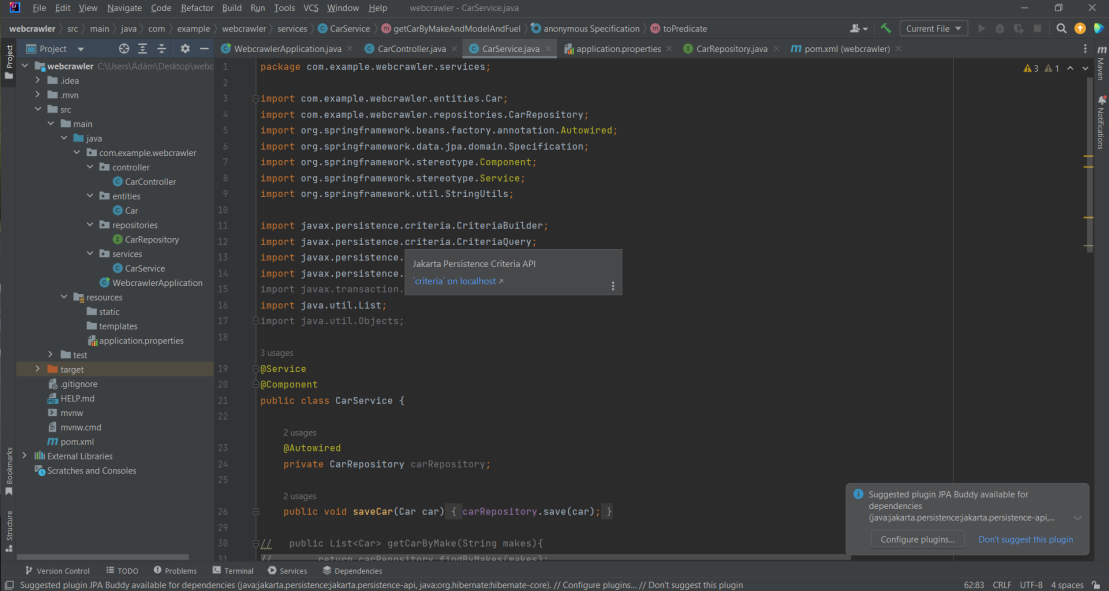
\includegraphics[scale=1]{images/Intelij.png}
\caption{Intelij IDEA felépítése.}
\label{fig:Intelij}
\end{figure}

\subsection{Visual Studio Code}

VS Code (\ref{fig:VSCode}. ábra) egy forráskód szerkesztő, amit a Microsoft fejlesztett ki 2015-ben \cite{VSCode}. Windows, Linux és MacOS operációs rendszereken érhető el. Nagyon sok programozási nyelvvel lehet használni, mint például:

\begin{itemize}
\item JavaScipt,
\item Go,
\item JavaScript,
\item C++,
\item Phyton.
\end{itemize}

Rengeteg kiegészítővel lehet bővíteni a fejlesztő környezetet, ami könnyebbé és átláthatóbbá teszi a fejlesztést, ezért esett a választásom erre a környezetre a frontend fejlesztéséhez.

\begin{figure}[h]
\centering
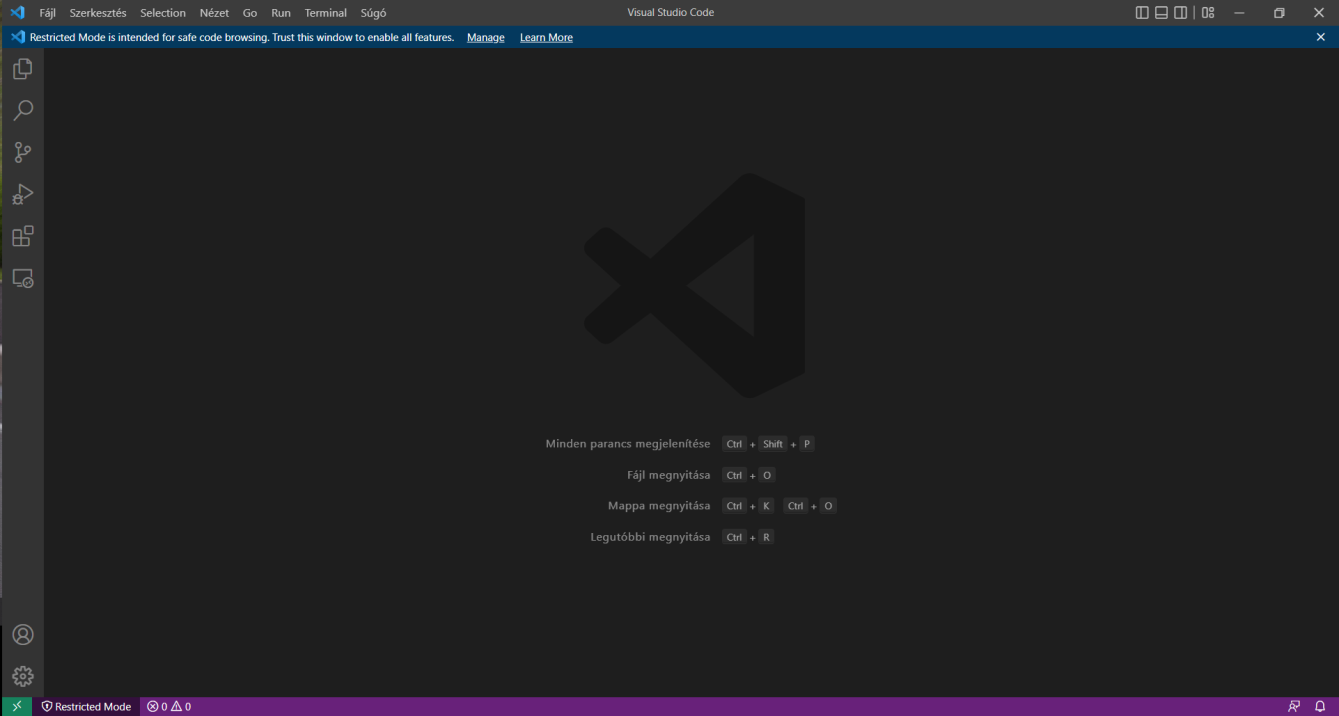
\includegraphics[scale=0.6]{images/VSCode.png}
\caption{Visual Studio Code képernyőkép.}
\label{fig:VSCode}
\end{figure}


\subsection{Postman}

A Postman \cite{Postman} API-k létrehozására és használatára, tesztelésére létrehozott platform. Használatával egyszerűbben és gyorsabban hozhatunk létre jobb minőségű API-kat. Rengetek eszközkészletet tartalmaz, amely tovább gyorsítja az API létrehozását a  tervezéstől egyenesen a tesztelésig. Ilyen eszközök a következők:

\begin{itemize}
\item API kliens: Lehetővé teszi API-k tesztelését, hibakeresését, és van lehetőség 
HT-
TP, REST, SOAP és GraphQL kéréseket is indítani.
\item API tervezés: OpenAPI, RAML, GraphQL vagy SOAP formátumban tervezhet-
jük meg az API-kat. A Postman Schema szerkesztője megkönnyíti a különböző méretű fájlokkal való munkát.
\item API dokumentáció: Postman automatikusan géppel olvasható dokumentációt hoz létre, amit OpenAPI-fájlokon keresztül dokumentál. Tartalmazza a kérések részle-
teit mintakódokkal.
\item API tesztelés: Lehetőség van használni funkcionális teszteket, integrációs teszte-
ket, regressziós teszteket. A Postman egy Node.js alapú futtatókörnyezet, ami támogatja gyakori tervezési mintákat és  könyvtárakat, ami segíti a gyors tesztké-
szítést.
\item Monitorozás: Naprakészek lehetünk az API állapotával és teljesítményével kap-csolatban. A monitorok a Postman felhőjében vannak tárolva, és ennek köszönhe-
tően gyorsan beállíthatjuk őket.
\item Mock szerverek: Más néven „Ál szerverek”, aminek segítségével láthatjuk, hogy hogyan fog futni az API-nk mielőtt kihelyeznénk az éles környezetbe. A Postman felhő üzemelteti, és így bárhonnan elérhetőek.
\end{itemize}

A \ref{fig:Postman}. ábrán látható a Postman-ről egy képernyőkép.

\begin{figure}[h]
\centering
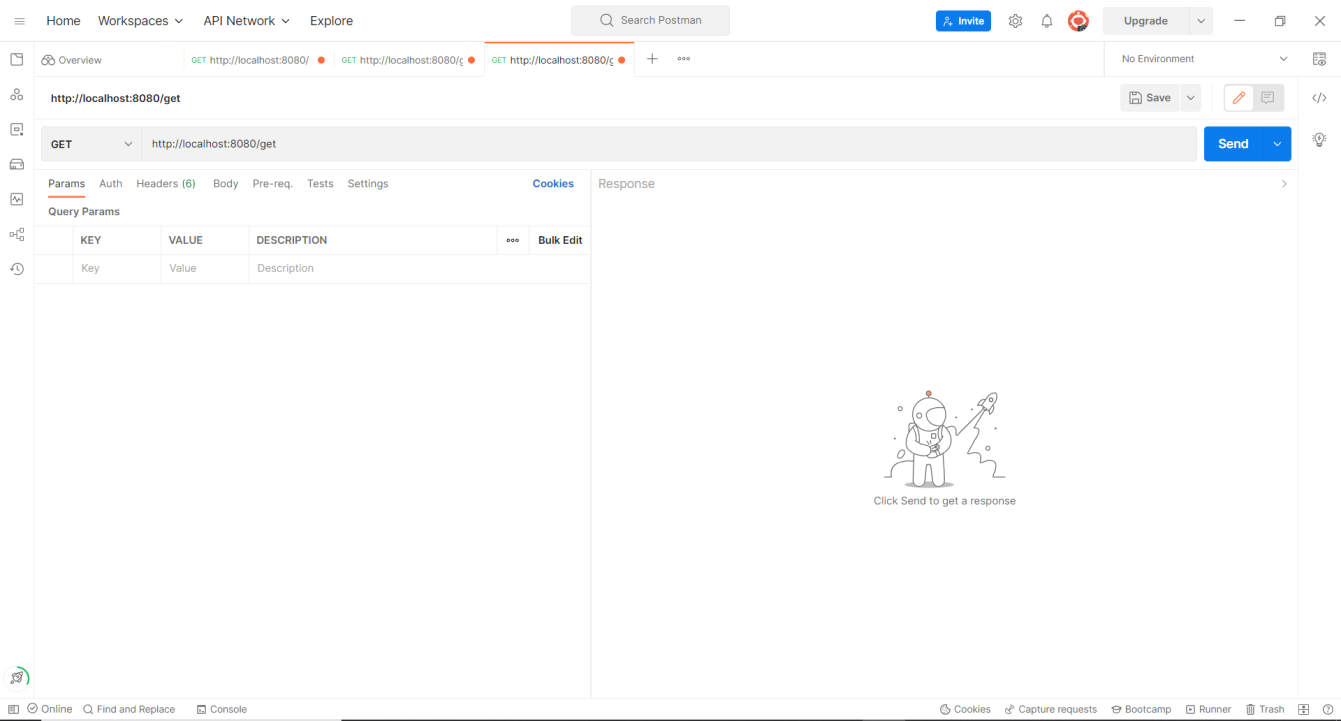
\includegraphics[scale=0.8]{images/Postman.png}
\caption{Postman URL tesztelője.}
\label{fig:Postman}
\end{figure}
\newpage

\subsection{PgAdmin}

A PgAdmin \cite{PgAdmin} egy grafikus felhasználói felület, ami a PostgreSQL kezelésére a lehető legjobb megoldás lehet, mert nagyon hatékonyan lehet vele dolgozni. Legújabb verziója a PgAdmin 4, amely jQuery, JavaScript és Python kombinációjával készült. Előnyei, hogy:

\begin{itemize}
\item kompatibilis Windows, Linux és MacOS operációs rendszerekkel is,
\item bárhova telepíthető ahol PostgreSQL-t használunk,
\item van olyan lekérdező eszköze, amivel gyorsabb az adatbevitel és a hibakezelés.
\end{itemize}

Rengeteg dokumentáció megtalálható hozzá amivel könnyedén el lehet kezdeni a használatát.

A \ref{fig:PgAdmin 4}. ábrán látható a PgAdmin 4 Dashboard-ja.

\begin{figure}[h]
\centering
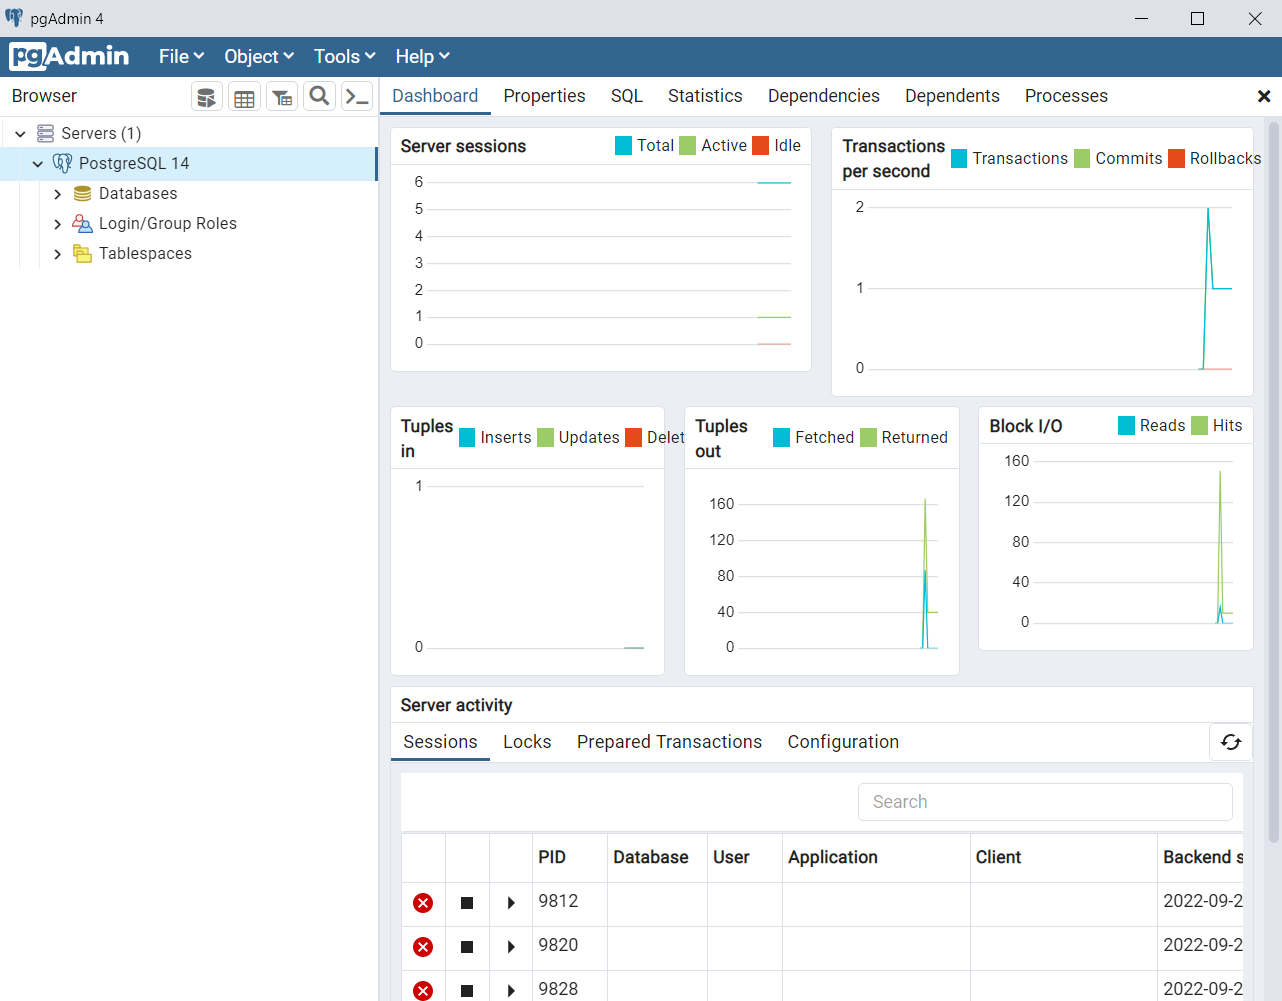
\includegraphics[scale=0.3]{images/PgAdmin.png}
\caption{PgAdmin 4 Dashboard.}
\label{fig:PgAdmin 4}
\end{figure}
\newpage

